\section{Klassendiagramm der Entwurfsphase}
\label{sec:anhang-klassendiagramm}

Aufgrund der Größe des Klassendiagramms wird dieses in drei Teilen dargestellt. Dabei sind diese in ihrer Reihenfolge entsprechend ihrer ursprünglichen Position im Gesamtmodell von links nach rechts zu betrachten.

\newcommand{\height}{16cm}

\begin{figure}
     \centering
     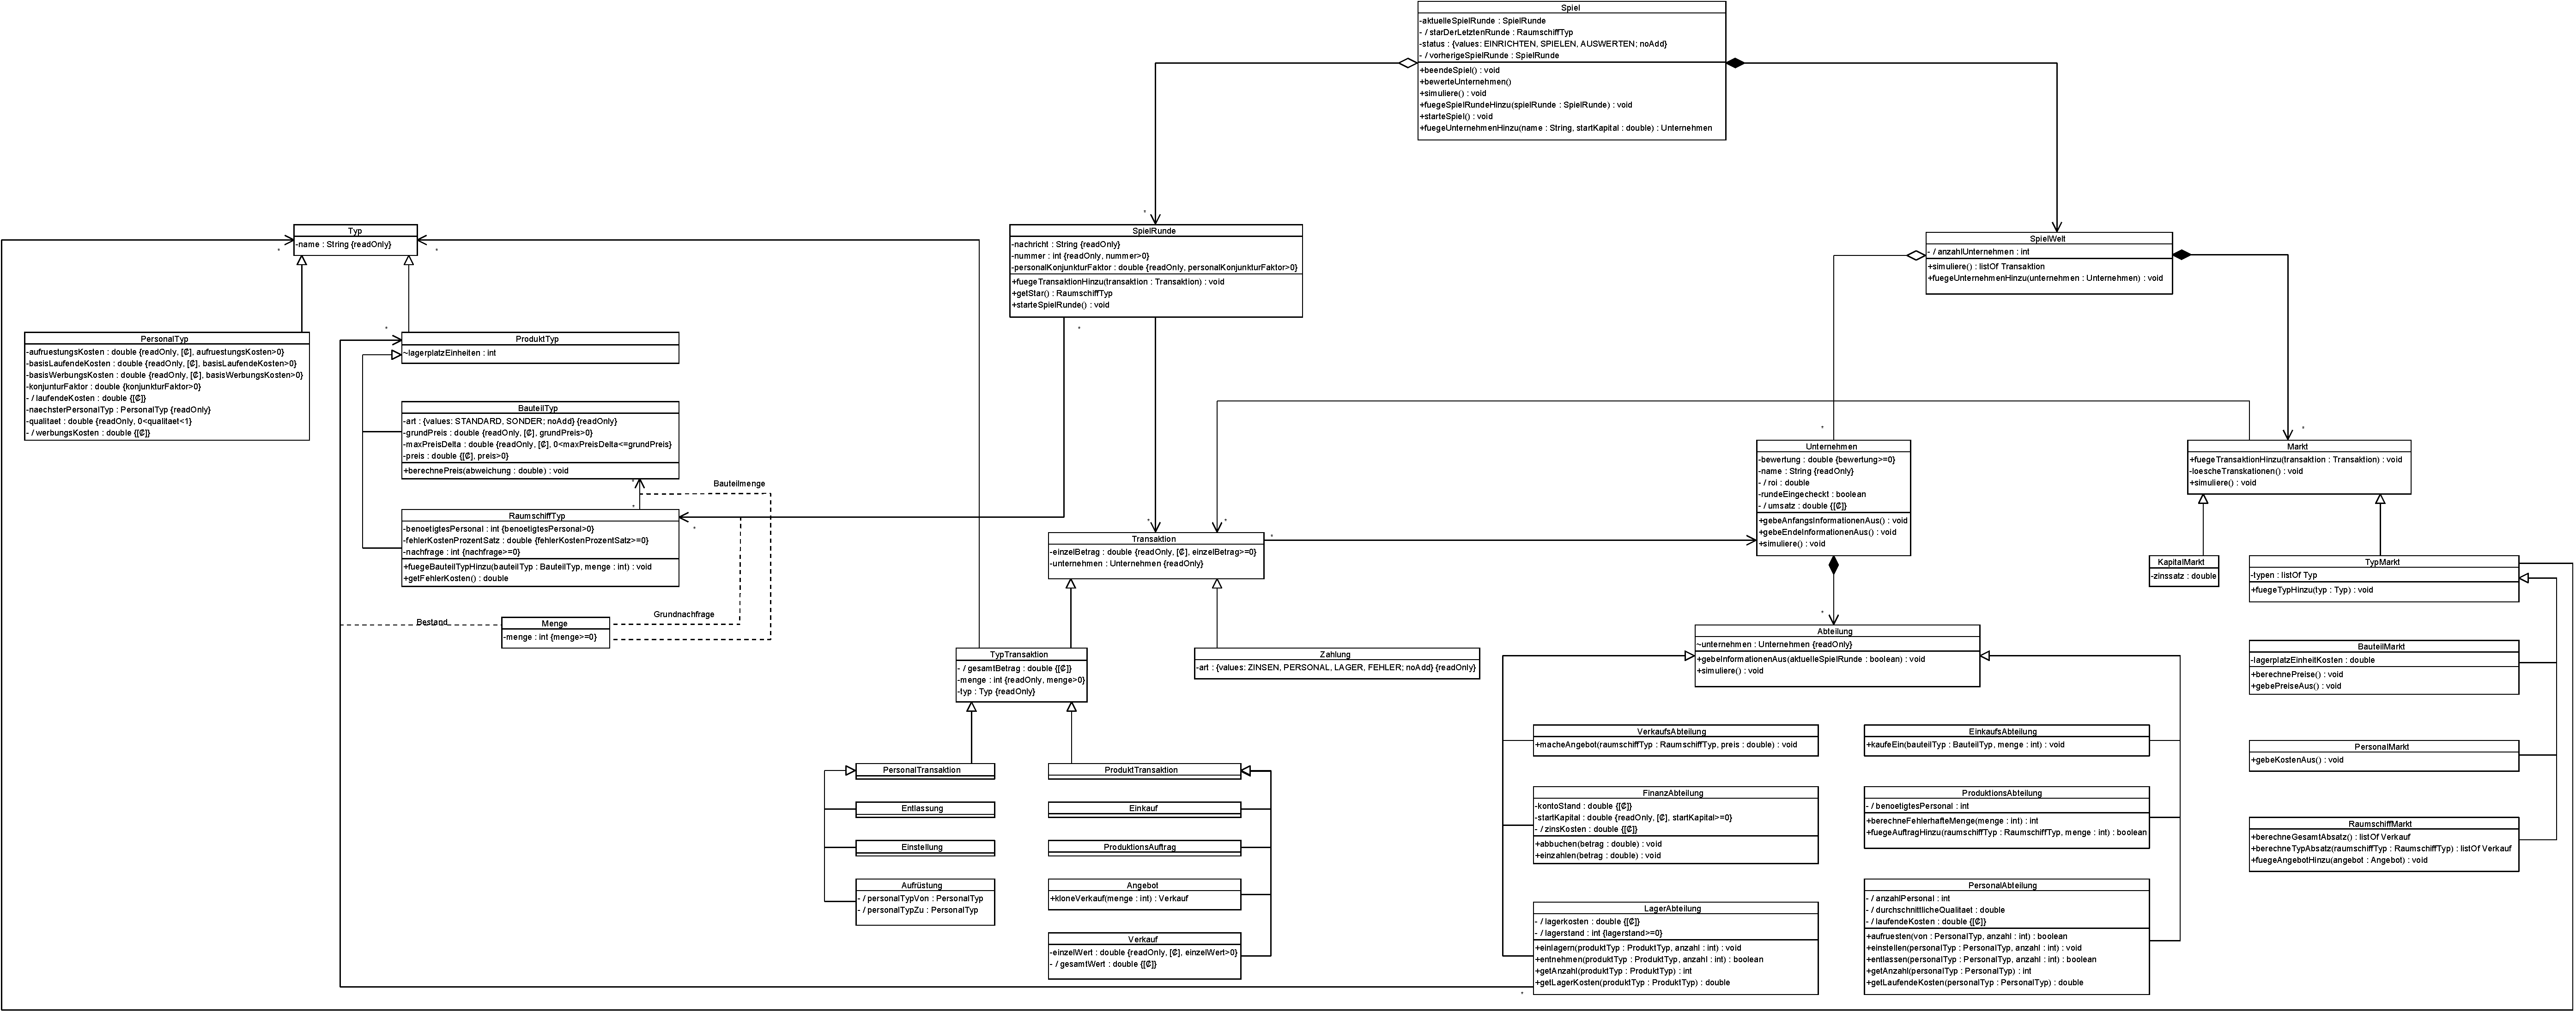
\includegraphics[height=\height,trim=0cm 0cm 66cm 0cm,clip=true]{70_Anhang/10_gesamtmodell}
\end{figure}

\begin{figure}
     \centering
     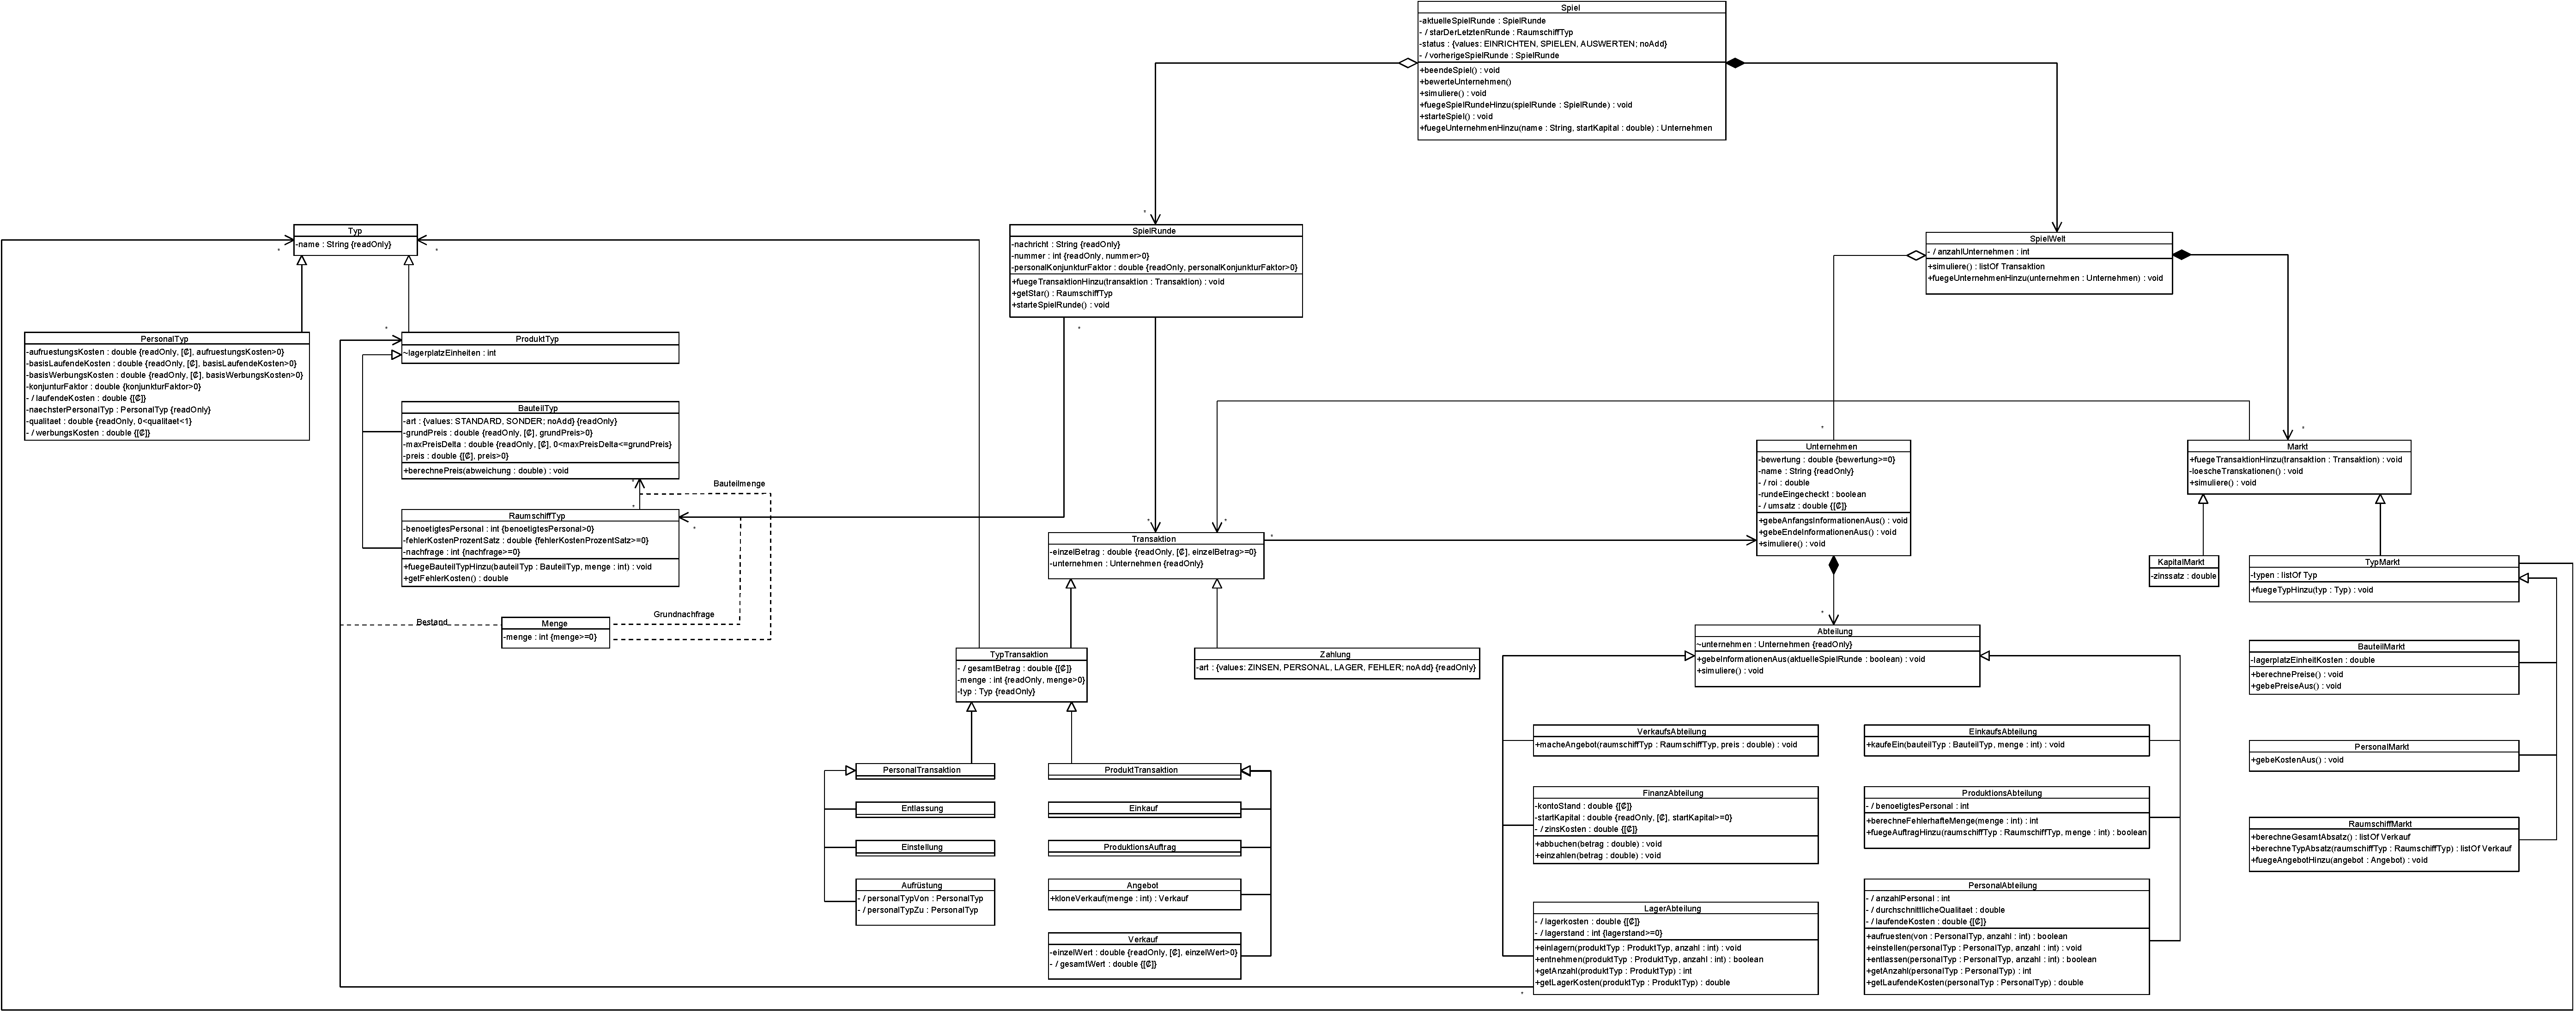
\includegraphics[height=\height,trim=30cm 0cm 30.2cm 0cm,clip=true]{70_Anhang/10_gesamtmodell}
\end{figure}

\begin{figure}
     \centering
     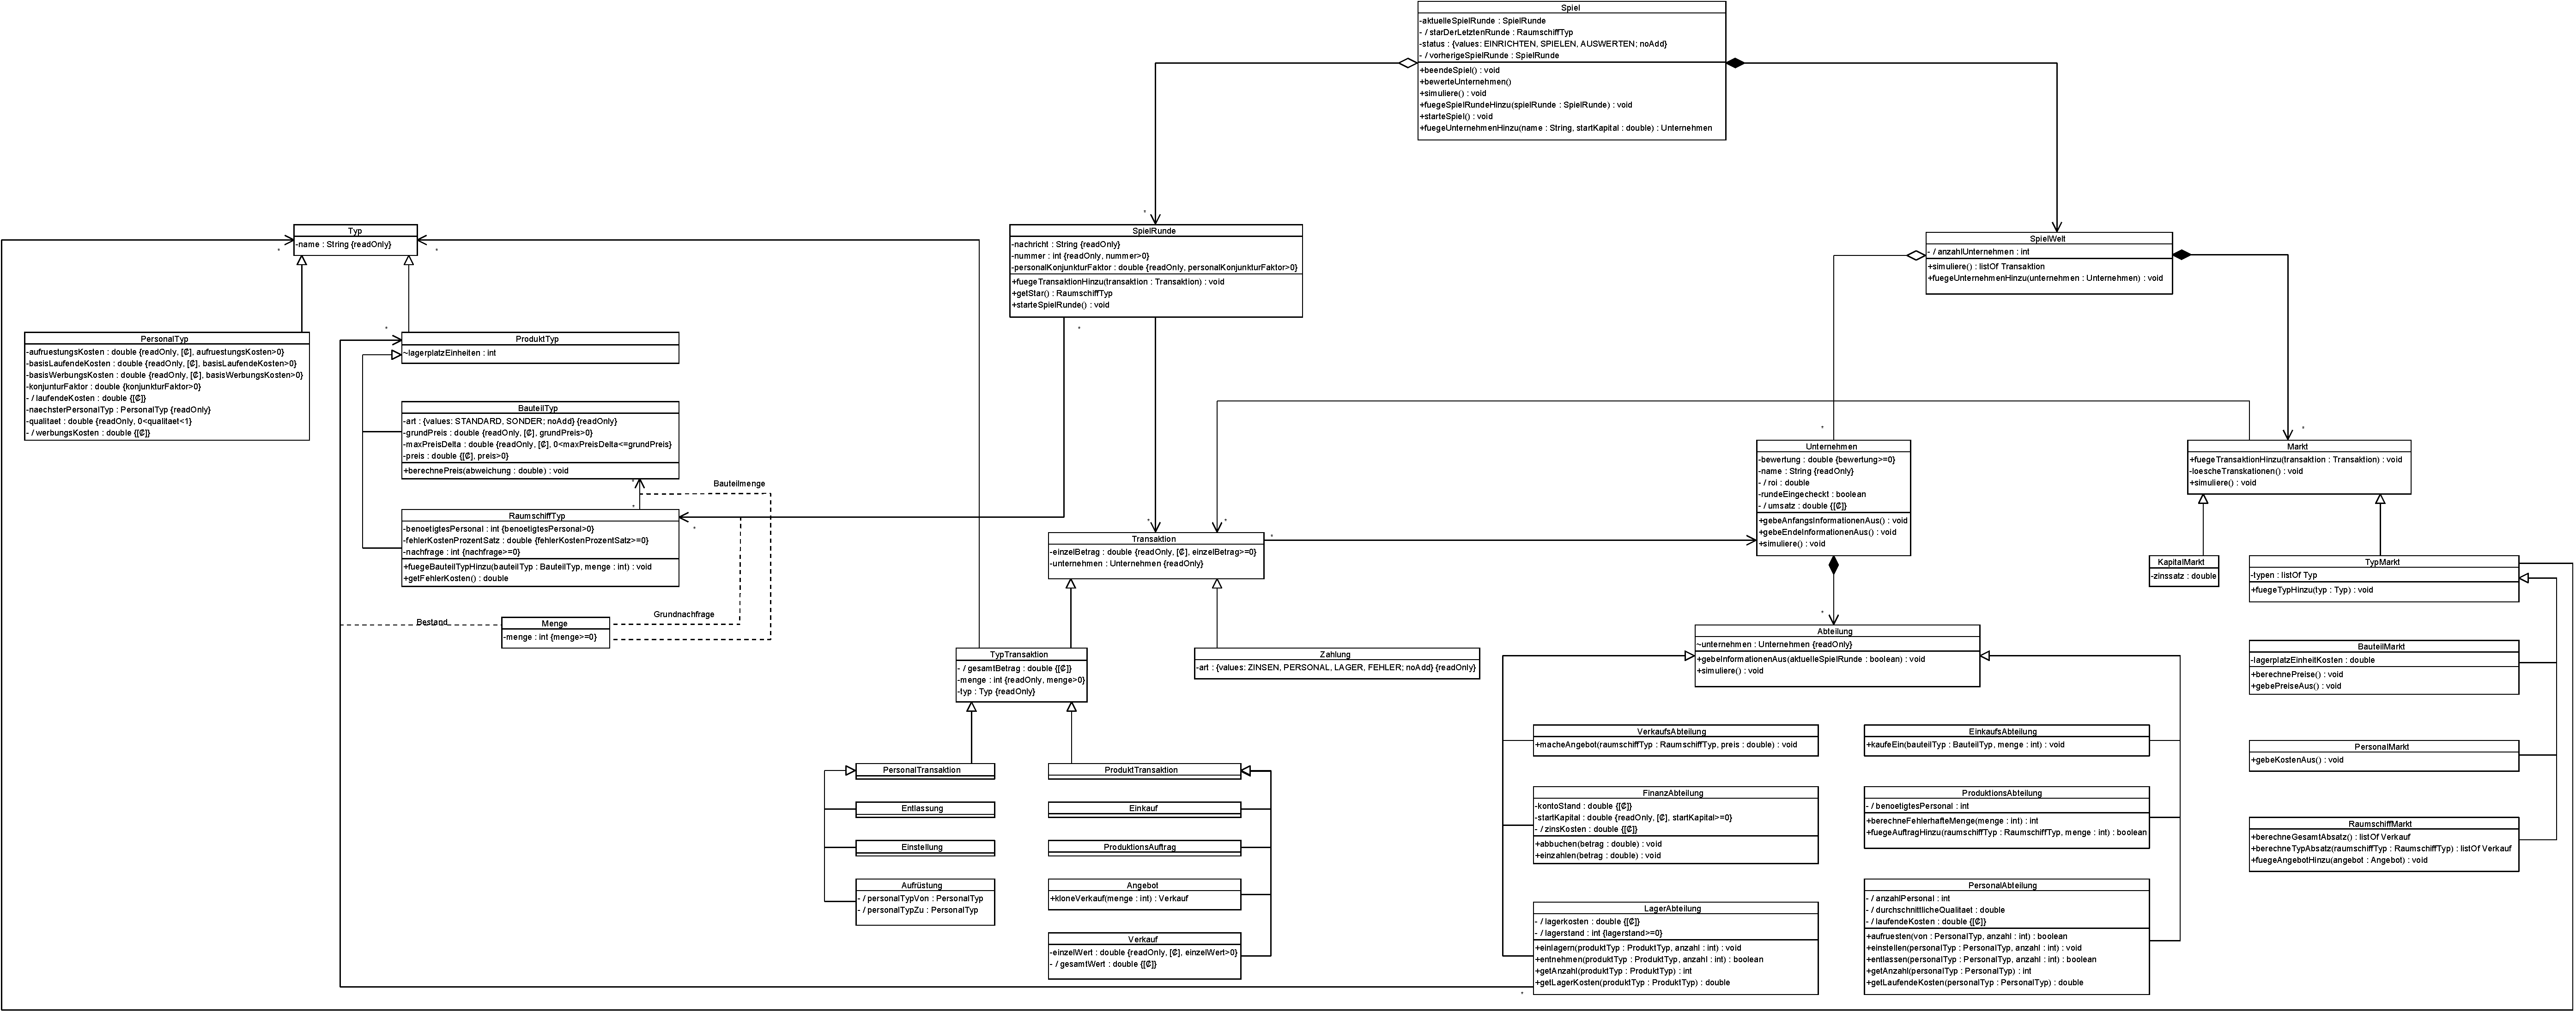
\includegraphics[height=\height,trim=55cm 0cm 0cm 0cm,clip=true]{70_Anhang/10_gesamtmodell}
\end{figure}